%===============================================================================
% $Id: ifacconf.tex 7 2007-11-21 12:50:23Z jpuente $
% Template for IFAC meeting papers
% Copyright (c) 2007 International Federation of Automatic Control
%===============================================================================
\documentclass{ifacconf}

\usepackage[round]{natbib} % you should have natbib.sty
\usepackage{graphicx}      % include this line if your document contains figures
\usepackage{amsmath}
\usepackage{booktabs}
%===============================================================================
\begin{document}
\begin{frontmatter}

\title{Nonlinear Control Applied to 4D Transport Aircraft Guidance} 
% Title, preferably not more than 10 words.


\author[First]{G. Sousa} 
%\author[Second]{Second B. Author, Jr.} 
%\author[Third]{Third C. Author}

\address[First]{Instituto Superior Técnico, Lisbon, Portugal (guilherme.sousa@ist.utl.pt
).}
%\address[Second]{Colorado State University, 
%   Fort Collins, CO 80523 USA (e-mail: author@lamar. colostate.edu)}
%\address[Third]{Electrical Engineering Department, 
%   Seoul National University, Seoul, Korea, (e-mail: author@snu.ac.kr)}

%%%%%%%%%%%%%%%%%%%%%%%%%%%%%%%%%%%%%%%%%%%%%%%%%%%%%%%%%%%%%%%%%%%%%%
%     File: ExtendedAbstract_abstr.tex                               %
%     Tex Master: ExtendedAbstract.tex                               %
%                                                                    %
%     Author: Andre Calado Marta                                     %
%     Last modified : 2 Dez 2011                                     %
%%%%%%%%%%%%%%%%%%%%%%%%%%%%%%%%%%%%%%%%%%%%%%%%%%%%%%%%%%%%%%%%%%%%%%
% The abstract of should have less than 500 words.
% The keywords should be typed here (three to five keywords).
%%%%%%%%%%%%%%%%%%%%%%%%%%%%%%%%%%%%%%%%%%%%%%%%%%%%%%%%%%%%%%%%%%%%%%

%%
%% Abstract
%%
\begin{abstract}

Following the current ATM industry paradigm shift to allow for commercial aircraft to follow 4D trajectory, in order to increase both safety and air capacity, a controller was design and implemented in this work to reach such a goal in cruise conditions. The control law used is based on feedback linearisation, and a neural network is also implemented in order to restrain errors caused by modelling uncertainties caused by poor estimation of the aircraft parameters, external disturbances or fault systems. The neural network is trained online using the back-propagation algorithm to optimise the nonlinear inversion, resulting in an overall adaptive model-based controller. Simulation results show this controller is able to maintain stability and controllability in conditions that would otherwise render the aircraft unstable.
\\
%%
%% Keywords (max 5)
%%
\noindent{{\bf Keywords:}} non-linear control, feedback linearisation, neural network, flight control, back-propagation \\

\end{abstract}



\end{frontmatter}
%===============================================================================

%%%%%%%%%%%%%%%%%%%%%%%%%%%%%%%%%%%%%%%%%%%%%%%%%%%%%%%%%%%%%%%%%%%%%%
%     File: ExtendedAbstract_intro.tex                               %
%     Tex Master: ExtendedAbstract.tex                               %
%                                                                    %
%     Author: Andre Calado Marta                                     %
%     Last modified : 27 Dez 2011                                    %
%%%%%%%%%%%%%%%%%%%%%%%%%%%%%%%%%%%%%%%%%%%%%%%%%%%%%%%%%%%%%%%%%%%%%%
% State the objectives of the work and provide an adequate background,
% avoiding a detailed literature survey or a summary of the results.
%%%%%%%%%%%%%%%%%%%%%%%%%%%%%%%%%%%%%%%%%%%%%%%%%%%%%%%%%%%%%%%%%%%%%%

\section{Introduction}
\label{sec:intro}

As the aeronautic industry grows, so is bound to also grow the air traffic dramatically. To answer this problematic ATM researchers have proposed over the last few years Trajectory-Based Operations (TBO), a concept allowing the use of 4D trajectories to manage both safety and air capacity. In both the US and Europe, initiatives to put such systems in place are currently being developed and implemented, namely the NextGen by the FAA and and SESAR EUROCONTROL. Therefore, in order to adopt this air traffic management paradigm, automation will play a crucial role in 4D guidance control, allowing an aircraft to follow flight plans more accurately.

In order to fully automatize a commercial aircraft to follow a 4D trajectory in cruise conditions, this work will focus on designing and implementing an autopilot capable of controlling the aircraft attitude, improving flight quality and stability in hazardous piloting situations, to be integrated in a Fly-by-Wire system. The ultimate aim of this project will be to focus on auto pilot to provide 4D trajectory guidance to a commercial aircraft. To do so a model based controller is used, unlike in the currently implemented framework of robust control composed of several PID layers. This model based controller distinguishes fast and slow dynamics, using a nonlinear inversion of the fast dynamics to determine the necessary deflections of the control surfaces. 

This method, however, also has some limitations, the main one being that the feedback linearisation requires an exact knowledge of the system model, to obtain an exact inversion of the system. This is not usually feasible, and errors in the model of the airplane will inevitably lead to inversion errors, especially in cases of heavy external disturbances. A solution for this limitation will be proposed, studied and implemented in this work. 

Over the recent years, research in intelligent and adaptive flight control systems has seen a consistent increase, in an attempt to solve these limitations, in order to develop flight systems able to adapt to external disturbances \cite{SotA_IFCS}. Of the existing intelligent control techniques used to solve the dependency of model-based control systems on an accurate mathematical model and the uncertainties caused by external disturbances or component failures, neural networks have been the most successful in doing so. Applied to UAV control, research works such as \cite{online_adaptiveNN}, \cite{UAV_adaptive}, \cite{UAV_adaptive2} and \cite{quad_NLI+NN} have showed neural networks can be used to increase flight control stability and and rendering flight systems adaptable to disturbances. For this work an online neural network was used to improve a model based flight controller of a commercial aircraft. 

This paper is organized as follows, Section 2  provides the mathematical model used as well as actuator dynamics. Section 3 focuses on the model-based approach used to control the aircraft, as well as a description on the neural network used to improve said control law. This section will also cover the implementation of the NN described previously and the guidance law used to ensure 4D trajectory following. Lastly Section 4 shows simulation results of the control approach, and conclusions are given in Section 5.
%%%%%%%%%%%%%%%%%%%%%%%%%%%%%%%%%%%%%%%%%%%%%%%%%%%%%%%%%%%%%%%%%%%%%%
%     File: ExtendedAbstract_backg.tex                               %
%     Tex Master: ExtendedAbstract.tex                               %
%                                                                    %
%     Author: Andre Calado Marta                                     %
%     Last modified : 27 Dez 2011                                    %
%%%%%%%%%%%%%%%%%%%%%%%%%%%%%%%%%%%%%%%%%%%%%%%%%%%%%%%%%%%%%%%%%%%%%%
% A Theory section should extend, not repeat, the background to the
% article already dealt with in the Introduction and lay the
% foundation for further work.
%%%%%%%%%%%%%%%%%%%%%%%%%%%%%%%%%%%%%%%%%%%%%%%%%%%%%%%%%%%%%%%%%%%%%%

\section{Flight Dynamics}
\label{sec:backg}

The work made in this article was built on top of the work done by \cite{hector} on 4D trajectory tracking. The model used in this work is a six degree of freedom transport aircraft that will be described in this section. 

\subsection{Frames of Reference}

The first step before describing the dynamics of a commercial aircraft will be to define the frames of reference used to do so. The first frame of reference, on which 4D trajectories are described, corresponds to the WGS84 frame of reference. A second frame of reference corresponding to the aircraft body frame will be used to provide its fast rotational dynamics. Lastly all aerodynamic forces will be applied in the axial directions of the wind frame. This frame is aligned to the wind speed vector relative to the airplane, given by both the angle of attack $\alpha$ and the sideslip angle $\beta$. For these last two frames of reference, a rotation matrix can be defined from the wind frame to the body frame by


\begin{equation}
R_{BW}=
\begin{bmatrix}
c_\alpha c_\beta & -c_\alpha s_\beta & -s_\alpha \\
s_\beta & c_\beta & 0 \\
s_\alpha c_\beta & -s_\alpha s_\beta & c_\alpha
\end{bmatrix}
\label{eq:wind2body}
\end{equation}

To describe the attitude of the plane Euler, roll, pitch and yaw angles, will also be used, namely $\phi\{-\pi,\pi\}$, $\theta \{-\dfrac{\pi}{2},\dfrac{\pi}{2}\}$, $\psi \{-\pi,\pi\}$. From these angles the rotation matrix from the body to the earth frame is given by

\begin{equation}
R_{EB}=
\begin{bmatrix}
c_\theta c_\psi & s_\phi s_\theta c_\psi - c_\phi s_\psi & c_\phi s_\theta c_\psi + s_\phi s_\psi \\
c_\theta c_\psi & s_\phi s_\theta s_\psi + c_\phi c_\psi & c_\phi s_\theta s_\psi - s_\phi c_\psi \\
-s_\theta & s_\phi c_\theta & c_\phi c_\theta
\end{bmatrix}
\label{eq:body2earth}
\end{equation}

\subsection{Fast Dynamics}

The considered actuators of the aircraft that control its attitude are given by the control surface deflection $\delta = [\delta_{ail} \delta_{ele} \delta_{rud}]^T$, each applying a torque along an axis of the body frame. These torques are given by

\begin{equation}
\begin{bmatrix}
L'\\
M\\
N
\end{bmatrix}
= \dfrac{1}{2}\rho S V_a^2\left(
\begin{bmatrix}
bC_l\\
\bar{c}C_m\\
bC_n
\end{bmatrix}
+ C_\delta \delta\right)
\label{eq:torque}
\end{equation}

where $\bar{c}$ and $b$ represent the wing mean chord and its span respectively, $C_\delta$ and the moment coefficients $[C_l C_m C_n]^T$ are given by

\begin{equation}
C_\delta = 
\begin{bmatrix}
bC_{l\delta_{ail}} & 0 & bC_{l\delta_{rud}} \\
0 & \bar{c}C_{m\delta_{ele}} & 0 \\
bC_{n\delta_{ail}} & 0 & bC_{n\delta_{rud}}\\
\end{bmatrix}
\label{eq:cdelta}
\end{equation}
\begin{equation}
\begin{bmatrix}
C_l\\
C_m\\
C_n
\end{bmatrix} 
=
\begin{bmatrix}
C_{l\beta} \beta + C_{l_p} p \dfrac{b}{2V_a} + C_{l_r} r \dfrac{b}{2V_a}\\
C_{m_0} + C_{m_\alpha} \alpha + C_{m_q} q \dfrac{\bar{c}}{2V_a}\\
C_{n\beta} \beta + C_{n_p} p \dfrac{b}{2V_a} + C_{n_r} r \dfrac{b}{2V_a}
\end{bmatrix}
\label{eq:cmoment}
\end{equation}
Where $p, q, r$ are the body angular rates ($\Omega = [p\quad q\quad  r]^T$) and $V_a$ is the airspeed. The method for obtaining of the coefficients of equation \ref{eq:cmoment} will be provided in the chapter to follow. Having defined the torques applied to the aircraft the rotational dynamics equation can now be stated as per \cite{hector}, $I$ being the aircraft inertial matrix.
\begin{subequations}
	\begin{equation}
		\dot{\Omega} = I^{-1} M_{ext} - I^{-1}\Omega \times (I\Omega)
	\end{equation}
	\begin{equation}
		\dot{\Omega} = 
		\dfrac{1}{2}\rho S I^{-1} V_a^2\left(
		\begin{bmatrix}
			bC_l\\
			\bar{c}C_m\\
			bC_n
		\end{bmatrix}
		+ C_\delta \delta\right)
		- I^{-1}\Omega \times (I\Omega)	
	\end{equation}

\label{eq:fast_dynamics}
\end{subequations}

These two equations can be rearranged to account for the effect of the wind, allowing further on to simulate the behaviour of the airplane in the presence of wind disturbances. Let $\vec{V_G} = [u \quad v \quad w]^T$ be the speed of the CG relative to the ground, $\vec{V}$ the speed of the CG relative to the air mass and $\vec{W}$ the speed of the wind relative to the ground, then as per \cite{Etkin+Reid} 
\begin{equation}
\vec{V_G} = \vec{V} + \vec{W} = 
\begin{bmatrix}
V_ac_\alpha c_\beta + V_{w_x}\\
V_as_\beta+V_{w_y}\\
V_as_\alpha c_\beta + V_{w_z}
\end{bmatrix}
\label{eq:windtriangle}
\end{equation}
and $\alpha$ and $\beta$ can be computed by 
\begin{subequations}
	\begin{equation}
		\alpha = arctan\left(\dfrac{w-V_{w_z}}{uV_{w_x}}\right)
		\label{eq:alpha}
	\end{equation}
	\begin{equation}
		\beta = arctan\left(\dfrac{v-V_{w_y}}{V_a}\right)
		\label{eq:beta}
	\end{equation}
\end{subequations}

From these three equations, differentiating \ref{eq:alpha} and \ref{eq:beta}, and from equation \ref{eq:windtriangle} and the translation dynamics equation \ref{eq:boddy_acc} comes that 

\begin{equation}
\begin{bmatrix}
\dot{\alpha}\\
\dot{\beta}\\
\dot{V_a}
\end{bmatrix}
= 
\begin{bmatrix}
H_{11} & H_{12} & H_{13}\\
H_{21} & 0 & H_{23}\\
H_{31} & H_{32} & H_{33}
\end{bmatrix}
\begin{bmatrix}
p\\
q\\
r
\end{bmatrix}
+
\begin{bmatrix}
Q_1\\
Q_2\\
Q_3
\end{bmatrix}
\label{eq:alphabetadot}
\end{equation}
Where the entries of the matrix are given IN ANNEX DO ANNEX


The forces in the air frame $F_{xa}, F_{ya}, F_{za}$ will be further detailed in the next section on translation dynamics. 

The angular rates are also related to the Euler angles. The relationship between the euler angles and the rotation rates is also one that will prove useful when implementing the model on a Matlab simulation, and is given by

\begin{equation}
\begin{bmatrix}
\dot{\phi}\\
\dot{\theta}\\
\dot{\psi}
\end{bmatrix}
=
\begin{bmatrix}
1 & tg_\theta s_\phi & tg_\theta c_\phi\\
0 & c_\phi & -s_\phi\\
0 & \dfrac{s_\phi}{c_\theta} & \dfrac{c_\phi}{c_\theta}
\end{bmatrix}
\begin{bmatrix}
p\\
q\\
r
\end{bmatrix}
\label{eq:euler2omega}
\end{equation}

\subsection{Translation Dynamics}
This subsection on the forces applied to aircraft, introducing a new actuation variable, the thrust force $T$. These forces are applied along the three axis of the wind frame, lift, drag and side force, given by
\begin{equation}
\begin{bmatrix}
D\\
Y\\
L
\end{bmatrix}
= \dfrac{1}{2} \rho SV_a^2
\begin{bmatrix}
C_D\\
C_Y\\
C_L
\end{bmatrix}
\label{eq:forces}
\end{equation}

Although aerodynamic forces are usually expressed on the wind frame, as the thrust is always applied along the $x$ axis of the body frame, it is necessary to rotate the aerodynamic forces to this frame. This way the sum of the airplane's forces can be obtained. 

\begin{equation}
\begin{bmatrix}
F_{xa}\\
F_{ya}\\
F_{za}
\end{bmatrix}
= R_{WB}
\begin{bmatrix}
-D\\
Y\\
-L
\end{bmatrix}
\label{eq:body_forces}
\end{equation}
From Newton's Second Law comes the aircraft acceleration

\begin{equation}
\begin{bmatrix}
\dot{u}\\
\dot{v}\\
\dot{w}
\end{bmatrix}
=
\begin{bmatrix}
\dfrac{1}{m}(F_{xa} + T) - gs_\theta +rv-qw\\
\dfrac{1}{m}F_{ya} + gc_\theta s_\phi + pw - ru\\
\dfrac{1}{m}F_{za} + gc_\theta c_\phi + qu - pv
\end{bmatrix}
\label{eq:boddy_acc}
\end{equation}

An expression in the Earth frame can also be obtained

\begin{equation}
\begin{bmatrix}
\ddot{x}_E\\
\ddot{y}_E\\
\ddot{z}_E
\end{bmatrix}
= \dfrac{1}{m} R_{BE}
\begin{bmatrix}
F_{xa}+T\\
F_{ya}\\
F_{za}
\end{bmatrix}
+
\begin{bmatrix}
0\\
0\\
g
\end{bmatrix}
\end{equation}

\subsection{Actuator Dynamics}

Finally, to simulate the delay response in actuation in order to have a realistic simulation, first order systems were introduced to the actuator dynamics as per \cite{hector}. For the control surfaces $\delta_i$, given a desired $\delta_i^d$ comes

\begin{equation}
\dot{\delta_i} = \dfrac{1}{\xi_i}(\delta_i^d-\delta_i)
\label{eq:actuator_dynamics}
\end{equation}

Similarly for thrust

\begin{equation}
\dot{T} = \dfrac{1}{\xi_T}(T^d-T)
\end{equation}

$\xi_i$ and $\xi_T$ being time constants. As the responsiveness of the resultant thrust will be much slower than that of the control surfaces, $\xi_T>>\xi_i$.
The chosen commercial aircraft that will be simulated is the Boeing 737-200, an aircraft with over 30 years of service for which some information of flight parameters is readily available, such as weight, wing span and mean chord. The simulation was made in a cruise flight environment, at $200$ m/s velocity at $10000$ m above the ground. The chosen inertial matrix for this aircraft is given by

\begin{equation}
\begin{bmatrix}
1278369.56 & 0 & -135588.17\\
0 & 3781267.79 & 0\\
-135588.17 & 0 & 4877649.98
\end{bmatrix}
kg.m^2
\end{equation}

The ISA atmospheric model was used to measure the air density at any given height.
\begin{table}[htbp]
  \centering
  \caption{Boeing 737-2 parameters}
    \begin{tabular}{rr}
    \toprule
    Weight $m$ & $52390$ kg \\
    Wing Span $b$ & $28.35$ m \\
    Wing Area $S$ & $102.0$ m$^{2}$ \\
    Wing mean chord $\bar{c}$ & $4.35$ m \\
    Length $l$ & $30.53$ m \\
    \bottomrule
    \end{tabular}%
  \label{tab:b737_parameters}
\end{table}%
The time constants used for the actuators was $\xi_{\delta_i}=50$ms and $\xi_T=4$s for the engines.

A simplified block diagram of the plane simulator is given by POR EM ANEXO
%%%%%%%%%%%%%%%%%%%%%%%%%%%%%%%%%%%%%%%%%%%%%%%%%%%%%%%%%%%%%%%%%%%%%%
%     File: ExtendedAbstract_imple.tex                               %
%     Tex Master: ExtendedAbstract.tex                               %
%                                                                    %
%     Author: Andre Calado Marta                                     %
%     Last modified : 27 Dez 2011                                    %
%%%%%%%%%%%%%%%%%%%%%%%%%%%%%%%%%%%%%%%%%%%%%%%%%%%%%%%%%%%%%%%%%%%%%%
% A Calculation section represents a practical development
% from a theoretical basis.
%%%%%%%%%%%%%%%%%%%%%%%%%%%%%%%%%%%%%%%%%%%%%%%%%%%%%%%%%%%%%%%%%%%%%%

\section{Implementation}
\label{sec:imple}

Place text here...


%%%%%%%%%%%%%%%%%%%%%%%%%%%%%%%%%%%%%%%%%%%%%%%%%%%%%%%%%%%%%%%%%%%%%%
\subsection{Feedback Linearisation}

More text...


%%%%%%%%%%%%%%%%%%%%%%%%%%%%%%%%%%%%%%%%%%%%%%%%%%%%%%%%%%%%%%%%%%%%%%
\subsection{Online Neural Network}

More text...

\subsection{Guidance Law}
%%%%%%%%%%%%%%%%%%%%%%%%%%%%%%%%%%%%%%%%%%%%%%%%%%%%%%%%%%%%%%%%%%%%%%
%     File: ExtendedAbstract_resul.tex                               %
%     Tex Master: ExtendedAbstract.tex                               %
%                                                                    %
%     Author: Andre Calado Marta                                     %
%     Last modified : 27 Dez 2011                                    %
%%%%%%%%%%%%%%%%%%%%%%%%%%%%%%%%%%%%%%%%%%%%%%%%%%%%%%%%%%%%%%%%%%%%%%
% Results
% Results should be clear and concise.
% Discussion
% This should explore the significance of the results of the work, not
% repeat them. A combined Results and Discussion section is often
% appropriate. Avoid extensive citations and discussion of published
% literature.
%%%%%%%%%%%%%%%%%%%%%%%%%%%%%%%%%%%%%%%%%%%%%%%%%%%%%%%%%%%%%%%%%%%%%%

\section{Results}
\label{sec:resul}

This section will focus in testing and comparing the control algorithm developed so far, with and without the online NN corrections. These results will mainly focus in comparing both performances when facing modelling errors and system failures.


%%%%%%%%%%%%%%%%%%%%%%%%%%%%%%%%%%%%%%%%%%%%%%%%%%%%%%%%%%%%%%%%%%%%%%
\subsection{Inversion Errors}

This error will be the most frequent when implementing such a controller, as some system parameters estimations may have considerable errors, namely the aircraft inertial matrix. Fortunately, the controller used is, as it will be demonstrated, tolerant to errors in the estimation of this parameter, but can result in an unstable system in extreme cases. To simulate estimation errors, the entries of the inertial matrix $A$,$B$,$C$ and $E$ were multiplied by a reducing factor $\zeta \in [0;1]$ when computing the nonlinear inversion in \ref{eq:control_law}. The inertial matrix used in this equation $I_{est}$ is therefore given by $I_{est} = \zeta I$.

In order to more accurately visualise the influence of the $\zeta$ coefficient on the NLI controller for this same case, several simulations were made for values of $\zeta$ from $0$ to $1$. For each simulation the mean error was computed, in order to obtain a plot of these errors for each of the three references. From Figure \ref{fig:xi_mean_error} can be concluded that the error becomes considerable $\zeta<0.05$ for a controller without neural network compensation. For a compensated adaptive controller however, it is noticeable that errors only become considerable at $\zeta<0.02$.

\begin{figure}[h]
\centering
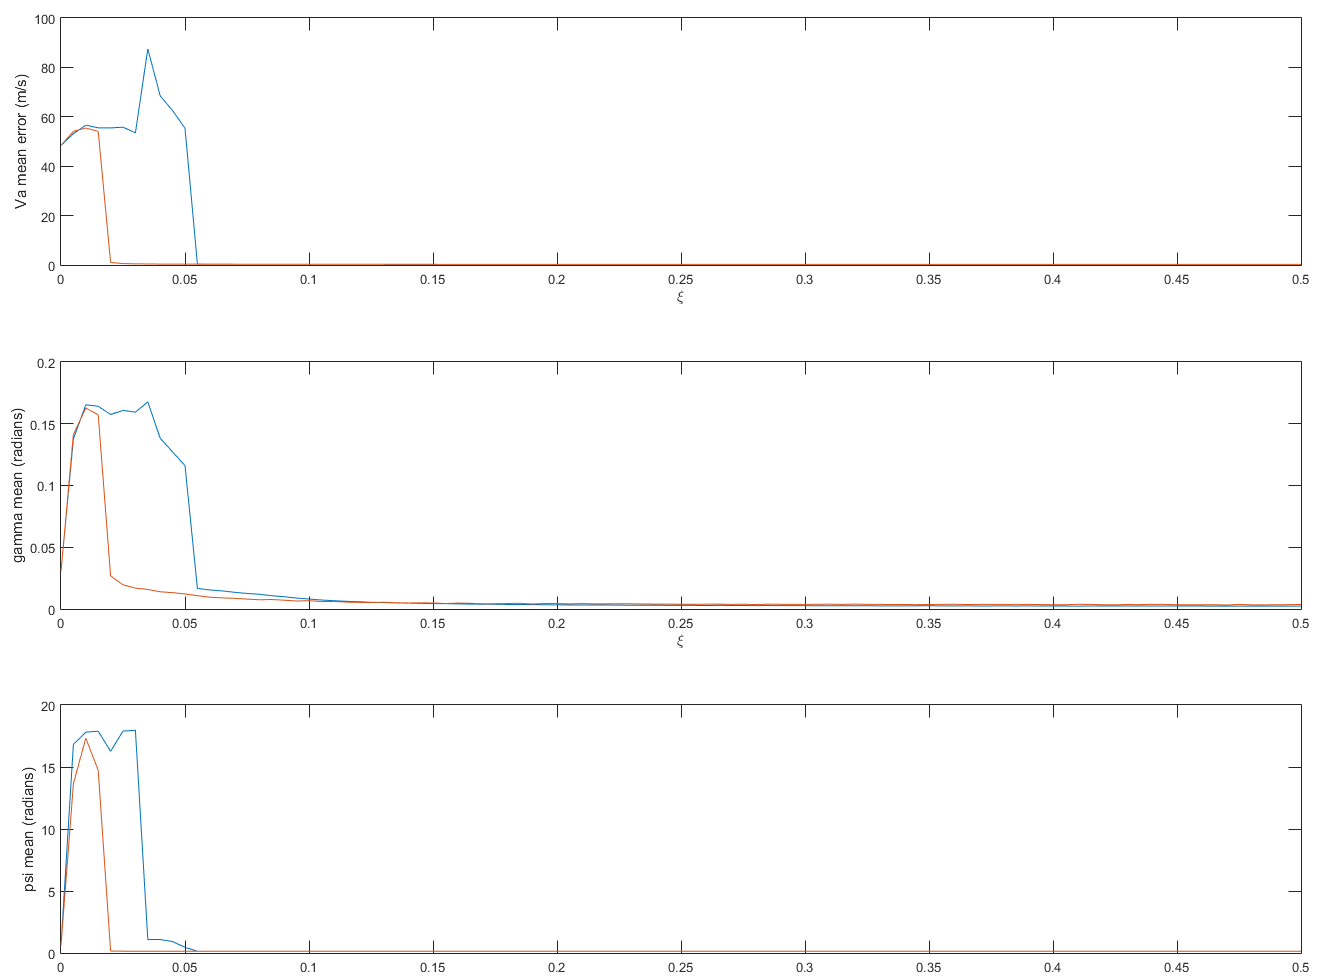
\includegraphics[width=0.5\textwidth]{../Figures/Results/mean_error_xi.png}
\caption[Mean errors for $V_a$, $\gamma$ and $psi$]{Mean errors for $V_a$, $\gamma$ and $psi$ for $\zeta=[0,0.5]$ with neural network compensation (orange) and without compensation (blue)}
\label{fig:xi_mean_error}
\end{figure}

\subsection{System Failures and External Disturbances}

One other cause for inversion errors that can have a much greater impact on flight trajectory are system failures. This subsection will focus on methods to simulate these failures and observe the behaviour of the airplane trajectory for these cases. The reference trajectory that will be used shall be the same as used previously. The first failure to be simulated will be a control surfaces failure, that will lead to reduced controllability of the aircraft. In this work this was replicated in a simulated environment by reducing by 80\% each moment coefficients for the elevator, aileron and rudder, namely $C_{\delta_{ele}}$, $C_{\delta_{ail}}$ and $C_{\delta_{rud}}$.

Applying the adaptive correction through the online neural network, the following trajectories were obtained

\begin{figure}[h]
\centering
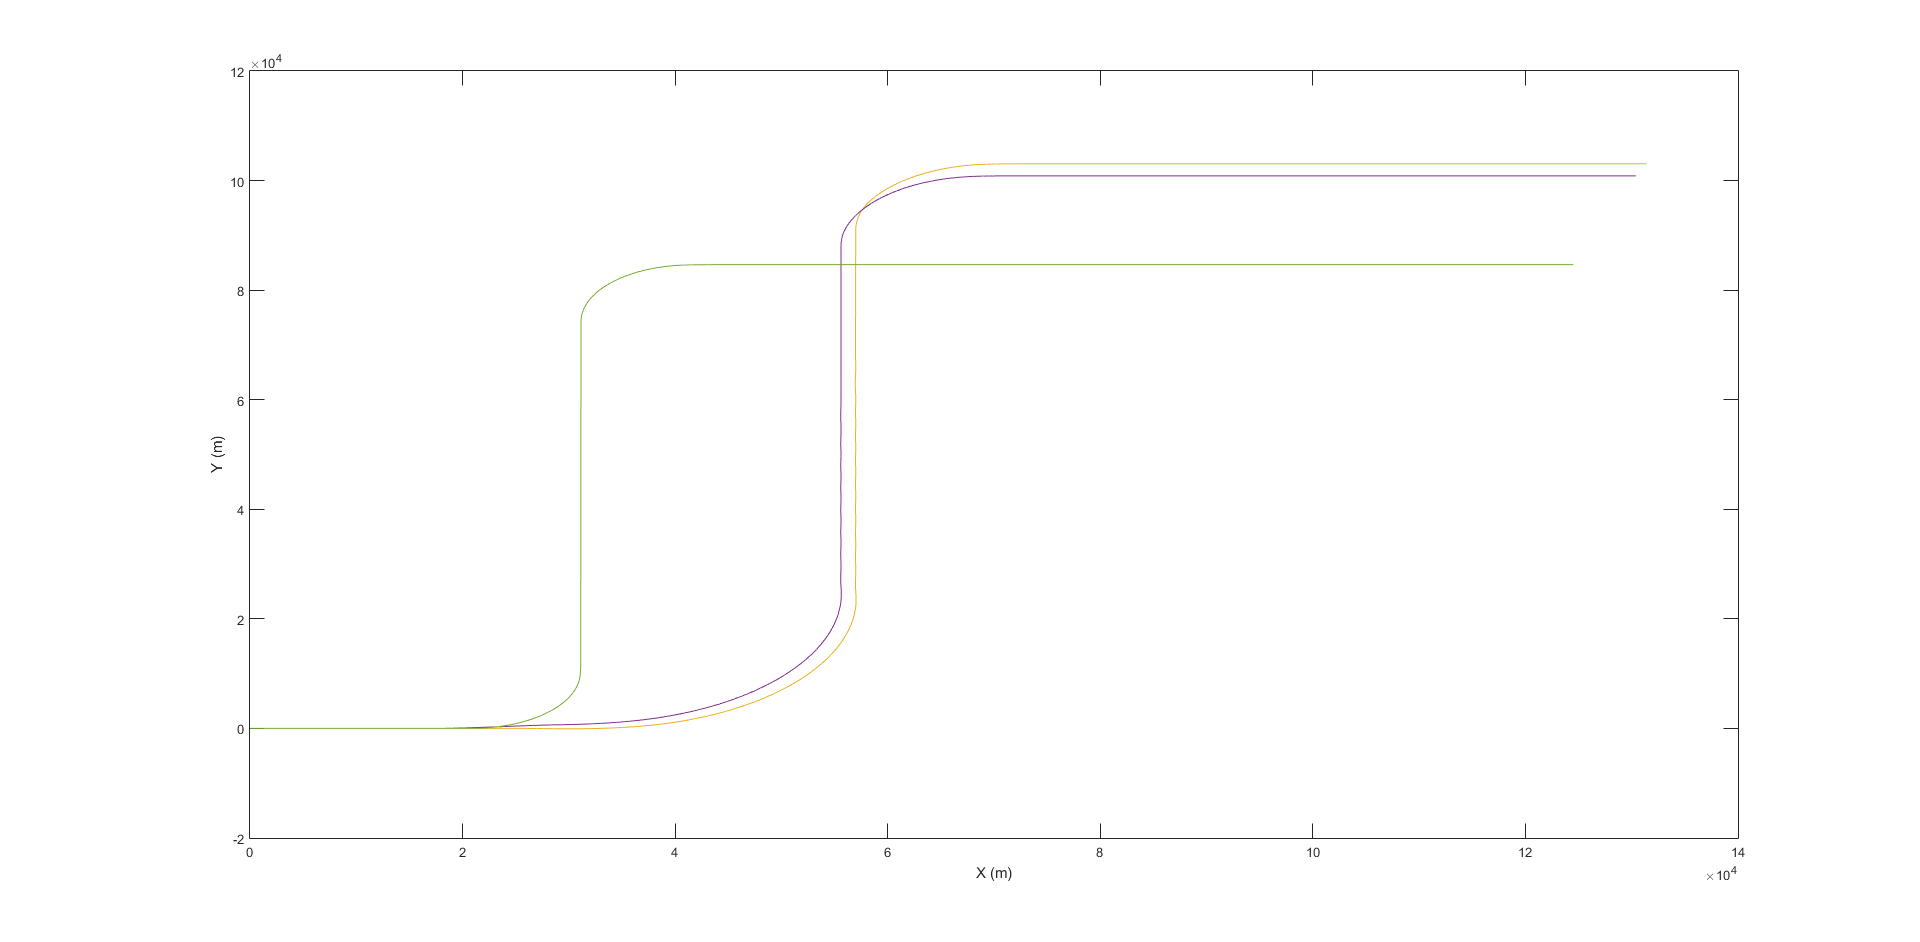
\includegraphics[width=0.5\textwidth]{../Figures/Results/reduced_act_NN.png}
\caption[Trajectory with reduced actuation corrected with NN correction]{Trajectory with 20\% reduced actuation (yellow) and trajectory without failures (green). The corrected trajectory by the NN can be seen in purple}
\label{fig:reduced_act_NN}
\end{figure}

The first observation that can be drawn from figure \ref{fig:reduced_act_NN} is that such an actuator failure severely reduces the controllability of the aircraft. 

The main consequence for this case will be, as could be expected, an increase in the convergence time to the desired heading. Note that the desired trajectory is not followed as this correction is only applied to the fast dynamics, and a guidance control law is not used. Comparing the two cases where the failures were implemented however, it can be observed that system corrected by the neural network converged to the desired heading slightly faster, resulting in a $2000m$ reduction in distance when comparing the non corrected control trajectory. 


%%%%%%%%%%%%%%%%%%%%%%%%%%%%%%%%%%%%%%%%%%%%%%%%%%%%%%%%%%%%%%%%%%%%%%
%     File: ExtendedAbstract_concl.tex                               %
%     Tex Master: ExtendedAbstract.tex                               %
%                                                                    %
%     Author: Andre Calado Marta                                     %
%     Last modified : 27 Dez 2011                                    %
%%%%%%%%%%%%%%%%%%%%%%%%%%%%%%%%%%%%%%%%%%%%%%%%%%%%%%%%%%%%%%%%%%%%%%
% The main conclusions of the study presented in short form.
%%%%%%%%%%%%%%%%%%%%%%%%%%%%%%%%%%%%%%%%%%%%%%%%%%%%%%%%%%%%%%%%%%%%%%

\section{Conclusions}
\label{sec:concl}

The nonlinear control law for fast dynamics was submitted to different types of perturbations and inversion errors. The controller showed to be robust to not only to errors in inertia estimation as well as small system failures. For more serious control perturbations however, the aircraft could not, as would be expected, follow the desired inputs. Using a $99.5\%$ smaller inertia relative to its true value in the NLI algorithm, increasing by $200\%$ the drag coefficient or by heavily reducing the ability of the control surfaces to influence the plane's dynamics, the aircraft's behaviour showed much higher reference tracking errors, sometimes even becoming uncontrollable. Concluding this first section the designed controller, using a model based approach, proved to be robust to most external perturbations and internal errors. 

Taking firstly the errors caused by errors in parameter estimations and gain tuning (for the linear law controlling the aircraft's model linearised by the FBL), the network showed improvements in robustness and reduced errors in airspeed and heading following, when compared to the same controller without the network. Similar tests were made with reduced control from actuators and in icing conditions. For the actuator failure case although the network slightly improve heading convergence times, reducing $C_{\delta_{ail}}, C_{\delta_{ele}}, C_{\delta_{rud}}$ by 80\% is still a too big perturbation for a commercial aircraft to recover from. For icing condition were simulated reduced lift coefficient, increased drag and reduced roll control ($C_{\delta_{ail}}$ was reduced by 30\%). For this case however, while the non corrected was unable to follow a heading and flight path angle references, this was not the case once the online neural network was added to the system. Indeed the network allowed the aircraft to follow a sinusoidal heading reference and to reduce the difference between $\gamma$ and its desired value. 

The same network architecture was used for all cases described above. Taking this into account it can be concluded that the goal of designing a neural network that would make the original NLI law more robust and able to adapt to different perturbations was indeed achieved.


\bibliography{ExtendedAbstract_ref_db}            

\appendix
 \section{$\dot{R_a}$ equation}
\label{sec:ra_dot}

\begin{gather*}
H_{11}=\dfrac{-V_a c_\alpha s_\beta  c_\beta - V_{w_y} c_\alpha c_\beta}{V_a(1+\tan^2\alpha)c^2_\alpha c^2_\beta}\\
H_{12}=\dfrac{V_a(c^2_\alpha c^2_\beta-s^2_\alpha c^2_\beta) + V_{w_x}c_\alpha c_\beta - V_{w_z}s_\alpha s_\beta}{V_a(1+\tan^2\alpha)c^2_\alpha c^2_\beta}\\
H_{13}=\dfrac{-V_a s_\alpha s_\beta  c_\beta - V_{w_y} s_\alpha c_\beta}{V_a(1+\tan^2\alpha)c^2_\alpha c^2_\beta}\\
H_{21}=\dfrac{V_a s_\alpha c_\beta + V_{w_z}}{V_a c_\beta}\\
H_{23}=-\dfrac{V_a c_\alpha c_\beta + V_{w_x}}{V_a c_\beta}\\
H_{31}=2 \left(-V_a s_\beta s_\alpha c_\beta - V_{w_x} s_\alpha c_\beta \right)\\
H_{32}=2\left( -V_{w_z} c_\alpha c_\beta + V_as_\alpha c_\beta s_\beta
 + V_{w_z}s_\beta + V_{w_x}s_\alpha c_\beta \right)\\
H_{33}=2\left(V_{w_y}c_\alpha c_\beta - V_{w_x}s_\beta\right)\\
Q_1=\dfrac{\left(\dfrac{1}{m}F_{za} + gc_\theta c_\phi - \dot{V}_{w_z} \right)c_\alpha c_\beta - \left(\dfrac{1}{m}(F_{xa} + T)-gs_\theta - \dot{V}_{w_x}\right)}{V_a(1+\tan^2\alpha)c^2_\alpha c^2_\beta}\\
Q_2=\dfrac{\dfrac{1}{m}F_{ya}+g c_\theta s_\phi-\dot{V}_{w_y}}{c_\beta}\\
Q_3=2 \left( \left(\dfrac{-1}{m}(F_{xa}+T) + g s_\theta - \dot{V}_{w_x} \right)c_\alpha c_\beta + \left( \dfrac{-1}{m}F_{ya} - \dot{V}_{w_y} \right)s_\beta \right.\\
\left. + \left(\dfrac{-1}{m}F_{za} - \dot{V}_{w_z} \right)s_\alpha c_\beta \right)
\label{eq:Ra_dot}
\end{gather*}

\end{document}
